In this section we first present a scheme for the fractional version of packing which does not assume the knowledge of $a^\ast(i,j)$. Later we present a second scheme that uses $a^\ast(i,j)$ and produces perfectly feasible solutions. Lastly we show how randomized  rounding is applied to both schemes by loosing $O(1)$ in the final objective.
\subsection{Scheme violating feasibility}
In \cite{buchbinder2009online} Buchbinder et al. proposed an online scheme for solving fractional packing with general coefficients.  Their scheme is $P$-competitive for any $P >0$ and results in a violation of the budget constraints as\\
$\sum_{i=1}^{|L|} \sum_{j=1}^{|R|} a(i,j)y(j) = B \times O(\frac{log n + log \frac{a_{max}}{a_{min}}}{P}) $,\\
where $a_{max}$ and $a_{min}$ are the maximum and minimum edge weights correspondingly.\\

We present the scheme in figure~\ref{fig:algo1}.\\
\begin{figure}[h]
  \centering
  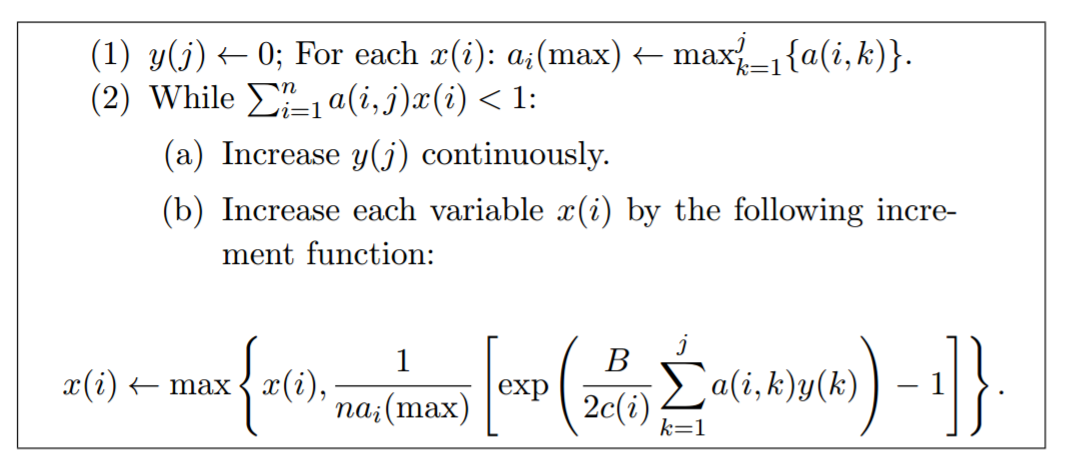
\includegraphics[width=3.3in]{figs/algo1.png}
  \caption{Online fractional packing - scheme 1}
  \label{fig:algo1}
\end{figure}
We also restate the main results from the paper which leads to the desired competitiveness of the scheme.
\begin{lemma}
\begin{itemize}
\ \\
(1) In each round $j$: $Y (j) \geq X(j)/P$.\\
(2) The primal solution produced by the scheme is feasible.\\
(3) For any dual constraint:\\
$\sum_{i=1}^{|L|} \sum_{j=1}^{|R|} a(i,j)y(j) \leq B \times \frac{2 log (1 + \frac{n a_{max}}{a_{min}})}{P}$ \ \\
$ = B \times O(\frac{log n + log \frac{a_{max}}{a_{min}}}{P})$
\end{itemize}
\end{lemma}
\subsection{Online ad-auction for slots}\label{sec:alg2}
We extend the algorithm proposed by buchbinder et al \cite{buchbinder2007online} for our problem as shown in algorithm \ref{alg:alg2}.
\begin{figure}[h]
  \centering
  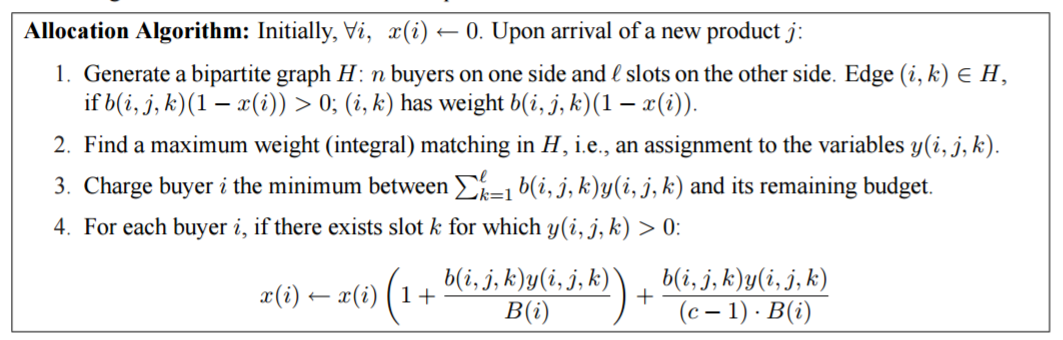
\includegraphics[width=3.3in]{figs/algo2.png}
  \caption{Online fractional ad-allocation - scheme 1}
  \label{fig:algo1}
\end{figure}
\ \\
However this only yields a fractional solution. We convert this to integral solution by a deterministic rounding, which ensures a $C$-competitive output.